% 测地线：曲面上连接 A、B 的"最直"曲线
\documentclass[border=4pt]{standalone}
\usepackage{tikz}
\usetikzlibrary{arrows.meta}
\usepackage{amsmath,amssymb}
\definecolor{fillA}{rgb}{0.45,0.45,0.45}
\definecolor{fillB}{rgb}{0.72,0.72,0.72}
\begin{document}
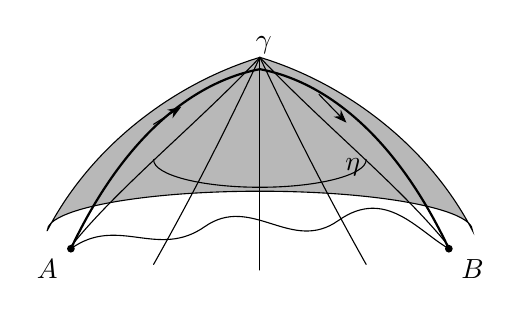
\begin{tikzpicture}[>=Stealth, line cap=round]
% 曲面（钟形）
\draw[fill=fillB] (0.6,1.15) .. controls (1.2,2.3) and (2.3,3.05) .. (3.3,3.35)
  .. controls (4.3,3.05) and (5.4,2.3) .. (6.0,1.15)
  arc (0:180:2.7 and 0.5) -- cycle;
% 经线与纬线
\draw (3.3,3.35) .. controls (2.5,2.5) and (1.5,1.7) .. (0.9,0.95);
\draw (3.3,3.35) .. controls (2.9,2.5) and (2.5,1.7) .. (1.95,0.72);
\draw (3.3,3.35) -- (3.3,0.65);
\draw (3.3,3.35) .. controls (3.7,2.5) and (4.1,1.7) .. (4.65,0.72);
\draw (3.3,3.35) .. controls (4.1,2.5) and (5.1,1.7) .. (5.7,0.95);
\draw (1.95,2.05) arc (180:360:1.35 and 0.35);
% 一般曲线 eta
\draw (0.9,0.92) .. controls (1.5,1.35) and (2.0,0.78) .. (2.6,1.2)
  .. controls (3.2,1.62) and (3.7,0.85) .. (4.3,1.28)
  .. controls (4.9,1.7) and (5.3,1.15) .. (5.7,0.92);
\node at (4.48,1.95) {$\eta$};
% 测地线 gamma（加粗）与切向量
\draw[thick] (0.9,0.92) .. controls (1.6,2.4) and (2.5,3.05) .. (3.3,3.2)
  .. controls (4.1,3.05) and (5.0,2.4) .. (5.7,0.92);
\node at (3.35,3.5) {$\gamma$};
\draw[->] (1.95,2.5) -- (2.3,2.72);
\draw[->] (4.05,2.88) -- (4.4,2.52);
% 端点
\fill (0.9,0.92) circle (1.4pt);
\fill (5.7,0.92) circle (1.4pt);
\node at (0.6,0.66) {$A$};
\node at (6.0,0.66) {$B$};
\end{tikzpicture}
\end{document}
